\documentclass[11pt,a4paper]{article}
\usepackage{fontspec}
\providecommand{\euro}{€}
\usepackage[british]{babel}
\usepackage[a4paper,margin=18mm,headheight=24pt]{geometry}
\usepackage{graphicx}
\usepackage[table]{xcolor}
\usepackage[most]{tcolorbox}
\usepackage{booktabs}
\usepackage{tabularx}
\usepackage{longtable}
\usepackage{xltabular}
\usepackage{array}
\usepackage[nobottomtitles*]{titlesec}
\usepackage{needspace}
\usepackage{fancyhdr}
\usepackage{fontawesome5}
\usepackage{etoolbox}
\usepackage[hidelinks]{hyperref}
\definecolor{sky}{HTML}{1C6DB4}
\definecolor{skyl}{HTML}{E6F0F8}
\definecolor{alert}{HTML}{B5382B}
\definecolor{alertl}{HTML}{FBE8EA}
\definecolor{summit}{HTML}{6B7A8F}
\definecolor{night}{HTML}{1B2A4A}
\definecolor{ink}{HTML}{1F2430}
\definecolor{or}{HTML}{B8860B}
\definecolor{orl}{HTML}{FBF3DC}
\AtBeginDocument{\color{ink}}
\titleformat{\section}{\Large\bfseries\sffamily\color{sky}}{}{0em}{}[{\vspace{1pt}\color{sky!35}\titlerule[1.1pt]}]
\titlespacing*{\section}{0pt}{14pt}{7pt}
\titleformat{\subsection}{\large\bfseries\sffamily\color{alert}}{}{0em}{}
\titlespacing*{\subsection}{0pt}{10pt}{4pt}
\pretocmd{\section}{\Needspace{10\baselineskip}}{}{}
\pretocmd{\subsection}{\Needspace{9\baselineskip}}{}{}
\widowpenalty=10000 \clubpenalty=10000 \raggedbottom
\setlength{\parindent}{0pt}\setlength{\parskip}{3pt}
\pagestyle{fancy}\fancyhf{}\renewcommand{\headrulewidth}{0.4pt}
\fancyhead[L]{\sffamily\small\color{night}\textbf{CELLAR INVENTORY}}
\fancyhead[R]{\sffamily\small\color{summit}VEND\'EMIAIRE}
\fancyfoot[C]{\sffamily\small\color{summit}\thepage}
\newtcolorbox{cadrebox}[1]{enhanced,unbreakable,colback=skyl,colframe=sky,coltitle=white,fonttitle=\bfseries\sffamily\small,boxrule=0.9pt,arc=2.5pt,title={\faClipboardList~~#1}}
\newtcolorbox{warnbox}[1]{enhanced,breakable,colback=alertl,colframe=alert,coltitle=white,fonttitle=\bfseries\sffamily\small,boxrule=0.9pt,arc=2.5pt,title={\faExclamationTriangle~~#1}}
\BeforeBeginEnvironment{cadrebox}{\par\Needspace{9\baselineskip}}
\begin{document}
\begin{titlepage}\centering\vspace*{30mm}

\includegraphics[width=42mm]{logo.png}\\[12mm]
{\sffamily\bfseries\fontsize{28}{34}\selectfont\color{night} Cellar inventory\par}\vspace{6mm}
{\sffamily\Large\color{sky} Insurance and inventory report\par}\vspace{14mm}
{\large\color{summit} October 26, 2026\par}
\vfill
{\small\color{summit} Vend\'emiaire\par}
\end{titlepage}
\section{Summary}
\begin{cadrebox}{Key figures}
\begin{tabularx}{\linewidth}{@{}Xr@{}}
Wines & \textbf{6} \\
Bottles & \textbf{20} \\
Stated value & \textbf{\euro{}745.86} \\
of which bottles valued (dated, sourced value) & 12 \\
of which bottles at purchase price & 8 \\
of which bottles with no known value & 0 \\
\end{tabularx}
\end{cadrebox}
Method: for each bottle, the latest value entered for this wine in this format, with its date and source; failing that, the purchase price (stated as such, at the purchase date); failing that, "not valued". The fill level uses the auction-house scale, with what it means for the age of the wine (sourced rules of the "Le vin" study).

\subsection{Weingut Sonnenhang · Kabinett · Mosel · 2016}
\begin{minipage}[t]{\linewidth}
{\color{summit}Mosel · Moselle · Allemagne · White}\par
Bottles : 4 — Stated value : \textbf{\euro{}76.40}
\end{minipage}\par\smallskip
{\footnotesize\begin{xltabular}{\linewidth}{@{}>{\raggedright\arraybackslash}p{0.22\linewidth}>{\raggedright\arraybackslash}X>{\raggedright\arraybackslash}p{0.17\linewidth}>{\raggedleft\arraybackslash}p{0.19\linewidth}@{}}
\toprule \textbf{Location, format, code} & \textbf{Fill level, condition, case, provenance} & \textbf{Purchase} & \textbf{Value (date, source)} \\ \midrule \endhead
---\newline Bottle\newline{\color{summit}\texttt{V50A25F4D1B}} & IN --- Into neck (Excellent for its age)\newline Label : Perfect\newline Capsule : Intact & \euro{}19.10 · January 18, 2025 · Caviste & \textbf{\euro{}19.10}\newline {\color{summit}purchase price, January 18, 2025} \\ \midrule[0.2pt]
---\newline Bottle\newline{\color{summit}\texttt{V113D163BE0}} & IN --- Into neck (Excellent for its age)\newline Label : Perfect\newline Capsule : Intact & \euro{}19.10 · January 18, 2025 · Caviste & \textbf{\euro{}19.10}\newline {\color{summit}purchase price, January 18, 2025} \\ \midrule[0.2pt]
---\newline Bottle\newline{\color{summit}\texttt{V2A1FF8C3C9}} & IN --- Into neck (Excellent for its age)\newline Label : Perfect\newline Capsule : Intact & \euro{}19.10 · January 18, 2025 · Caviste & \textbf{\euro{}19.10}\newline {\color{summit}purchase price, January 18, 2025} \\ \midrule[0.2pt]
---\newline Bottle\newline{\color{summit}\texttt{V3851591093}} & IN --- Into neck (Excellent for its age)\newline Label : Perfect\newline Capsule : Intact & \euro{}19.10 · January 18, 2025 · Caviste & \textbf{\euro{}19.10}\newline {\color{summit}purchase price, January 18, 2025} \\ \midrule[0.2pt]
\bottomrule\end{xltabular}}
\subsection{Weingut Sonnenhang · Kabinett · Mosel · 2024}
\begin{minipage}[t]{\linewidth}
{\color{summit}Mosel · Moselle · Allemagne · White}\par
Bottles : 4 — Stated value : \textbf{\euro{}140}
\end{minipage}\par\smallskip
{\footnotesize\begin{xltabular}{\linewidth}{@{}>{\raggedright\arraybackslash}p{0.22\linewidth}>{\raggedright\arraybackslash}X>{\raggedright\arraybackslash}p{0.17\linewidth}>{\raggedleft\arraybackslash}p{0.19\linewidth}@{}}
\toprule \textbf{Location, format, code} & \textbf{Fill level, condition, case, provenance} & \textbf{Purchase} & \textbf{Value (date, source)} \\ \midrule \endhead
---\newline Bottle\newline{\color{summit}\texttt{V5C328B1062}} & IN --- Into neck (Excellent for its age)\newline Label : Slightly damaged\newline Capsule : Intact\newline Carton & \euro{}23.45 · April 11, 2018 · Foire aux vins & \textbf{\euro{}35}\newline {\color{summit}estimation (démonstration), September 26, 2026} \\ \midrule[0.2pt]
---\newline Bottle\newline{\color{summit}\texttt{V4B40BDD3FC}} & IN --- Into neck (Excellent for its age)\newline Label : Slightly damaged\newline Capsule : Intact\newline Carton & \euro{}23.45 · April 11, 2018 · Foire aux vins & \textbf{\euro{}35}\newline {\color{summit}estimation (démonstration), September 26, 2026} \\ \midrule[0.2pt]
---\newline Bottle\newline{\color{summit}\texttt{V67AAAF8DD5}} & IN --- Into neck (Excellent for its age)\newline Label : Slightly damaged\newline Capsule : Intact\newline Carton & \euro{}23.45 · April 11, 2018 · Foire aux vins & \textbf{\euro{}35}\newline {\color{summit}estimation (démonstration), September 26, 2026} \\ \midrule[0.2pt]
---\newline Bottle\newline{\color{summit}\texttt{V67256C8A1C}} & IN --- Into neck (Excellent for its age)\newline Label : Slightly damaged\newline Capsule : Intact\newline Carton & \euro{}23.45 · April 11, 2018 · Foire aux vins & \textbf{\euro{}35}\newline {\color{summit}estimation (démonstration), September 26, 2026} \\ \midrule[0.2pt]
\bottomrule\end{xltabular}}
\subsection{Bodegas Peña Alta · Reserva · Rioja · 2008}
\begin{minipage}[t]{0.22\linewidth}\vspace{0pt}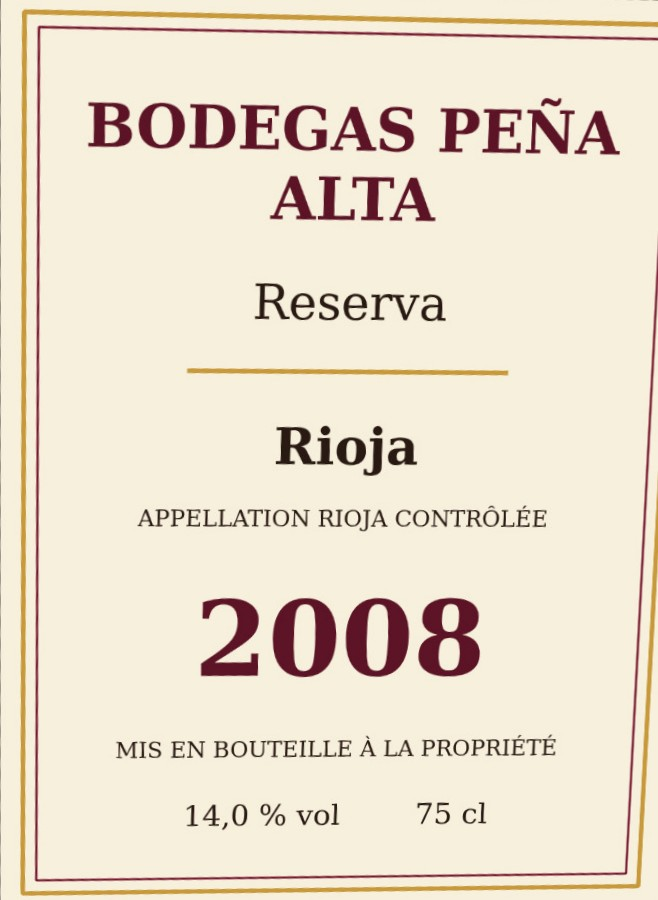
\includegraphics[width=\linewidth,height=42mm,keepaspectratio]{photo49.jpg}\end{minipage}\hfill\begin{minipage}[t]{0.75\linewidth}\vspace{0pt}
{\color{summit}Rioja · Rioja · Espagne · Red}\par
Bottles : 5 — Stated value : \textbf{\euro{}200}
\end{minipage}\par\smallskip
{\footnotesize\begin{xltabular}{\linewidth}{@{}>{\raggedright\arraybackslash}p{0.22\linewidth}>{\raggedright\arraybackslash}X>{\raggedright\arraybackslash}p{0.17\linewidth}>{\raggedleft\arraybackslash}p{0.19\linewidth}@{}}
\toprule \textbf{Location, format, code} & \textbf{Fill level, condition, case, provenance} & \textbf{Purchase} & \textbf{Value (date, source)} \\ \midrule \endhead
Cave de la maison › Mur nord › Casier A (row 2, column 2)\newline Bottle\newline{\color{summit}\texttt{VECFF20D6F6}} & IN --- Into neck (Excellent for its age)\newline Label : Slightly damaged\newline Capsule : Intact\newline Carton & \euro{}24.70 · January 10, 2021 · Au domaine & \textbf{\euro{}40}\newline {\color{summit}estimation (démonstration), September 26, 2026} \\ \midrule[0.2pt]
Cave de la maison › Mur nord › Casier A (row 6, column 2)\newline Bottle\newline{\color{summit}\texttt{VAC99A5767E}} & IN --- Into neck (Excellent for its age)\newline Label : Slightly damaged\newline Capsule : Intact\newline Carton & \euro{}24.70 · January 10, 2021 · Au domaine & \textbf{\euro{}40}\newline {\color{summit}estimation (démonstration), September 26, 2026} \\ \midrule[0.2pt]
Cave de la maison › Mur nord › Casier A (row 4, column 5)\newline Bottle\newline{\color{summit}\texttt{V7DA9DDB285}} & IN --- Into neck (Excellent for its age)\newline Label : Slightly damaged\newline Capsule : Intact\newline Carton & \euro{}24.70 · January 10, 2021 · Au domaine & \textbf{\euro{}40}\newline {\color{summit}estimation (démonstration), September 26, 2026} \\ \midrule[0.2pt]
Cave de la maison › Mur nord › Casier A (row 2, column 3)\newline Bottle\newline{\color{summit}\texttt{VC480E4F282}} & IN --- Into neck (Excellent for its age)\newline Label : Slightly damaged\newline Capsule : Intact\newline Carton & \euro{}24.70 · January 10, 2021 · Au domaine & \textbf{\euro{}40}\newline {\color{summit}estimation (démonstration), September 26, 2026} \\ \midrule[0.2pt]
Cave de la maison › Mur nord › Casier A (row 1, column 9)\newline Bottle\newline{\color{summit}\texttt{V1AB820A018}} & IN --- Into neck (Excellent for its age)\newline Label : Slightly damaged\newline Capsule : Intact\newline Carton & \euro{}24.70 · January 10, 2021 · Au domaine & \textbf{\euro{}40}\newline {\color{summit}estimation (démonstration), September 26, 2026} \\ \midrule[0.2pt]
\bottomrule\end{xltabular}}
\subsection{Domaine Weinberg-Hoff · Grand cru Schlossberg · Alsace grand cru · 2006}
\begin{minipage}[t]{\linewidth}
{\color{summit}Alsace grand cru · Alsace · France · White}\par
Bottles : 3 — Stated value : \textbf{\euro{}114}
\end{minipage}\par\smallskip
{\footnotesize\begin{xltabular}{\linewidth}{@{}>{\raggedright\arraybackslash}p{0.22\linewidth}>{\raggedright\arraybackslash}X>{\raggedright\arraybackslash}p{0.17\linewidth}>{\raggedleft\arraybackslash}p{0.19\linewidth}@{}}
\toprule \textbf{Location, format, code} & \textbf{Fill level, condition, case, provenance} & \textbf{Purchase} & \textbf{Value (date, source)} \\ \midrule \endhead
Cave de la maison › Mur nord › Casier B (row 6, column 4)\newline Bottle\newline{\color{summit}\texttt{V15C199CBAF}} & VTS --- Very top shoulder (Excellent for its age)\newline Label : Perfect\newline Capsule : Intact\newline Carton & \euro{}31.19 · May 1, 2026 · Salon des vins & \textbf{\euro{}38}\newline {\color{summit}estimation (démonstration), September 26, 2026} \\ \midrule[0.2pt]
Cave de la maison de montagne › Étagère › Rayonnage (row 2, column 5)\newline Bottle\newline{\color{summit}\texttt{VB41EEEE927}} & VTS --- Very top shoulder (Excellent for its age)\newline Label : Perfect\newline Capsule : Intact\newline Carton & \euro{}31.19 · May 1, 2026 · Salon des vins & \textbf{\euro{}38}\newline {\color{summit}estimation (démonstration), September 26, 2026} \\ \midrule[0.2pt]
Cave de la maison › Mur nord › Casier A (row 3, column 9)\newline Bottle\newline{\color{summit}\texttt{VEAC649AB04}} & VTS --- Very top shoulder (Excellent for its age)\newline Label : Perfect\newline Capsule : Intact\newline Carton & \euro{}31.19 · May 1, 2026 · Salon des vins & \textbf{\euro{}38}\newline {\color{summit}estimation (démonstration), September 26, 2026} \\ \midrule[0.2pt]
\bottomrule\end{xltabular}}
\subsection{Domaine du Grand Mûrier · Morgon · 2024}
\begin{minipage}[t]{0.22\linewidth}\vspace{0pt}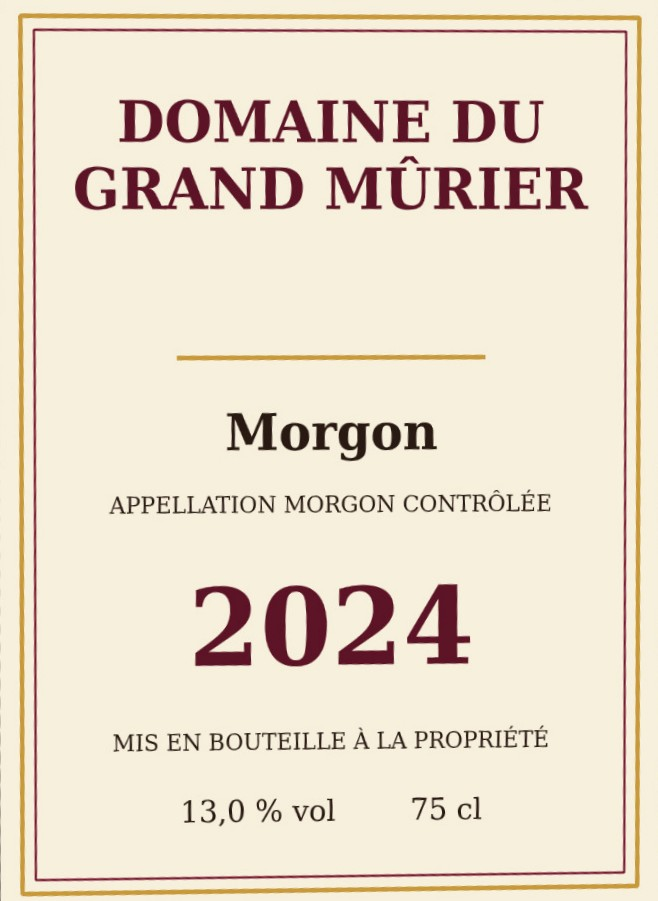
\includegraphics[width=\linewidth,height=42mm,keepaspectratio]{photo22.jpg}\end{minipage}\hfill\begin{minipage}[t]{0.75\linewidth}\vspace{0pt}
{\color{summit}Morgon · Beaujolais · France · Red}\par
Bottles : 2 — Stated value : \textbf{\euro{}37.06}
\end{minipage}\par\smallskip
{\footnotesize\begin{xltabular}{\linewidth}{@{}>{\raggedright\arraybackslash}p{0.22\linewidth}>{\raggedright\arraybackslash}X>{\raggedright\arraybackslash}p{0.17\linewidth}>{\raggedleft\arraybackslash}p{0.19\linewidth}@{}}
\toprule \textbf{Location, format, code} & \textbf{Fill level, condition, case, provenance} & \textbf{Purchase} & \textbf{Value (date, source)} \\ \midrule \endhead
Cave de la maison › Armoire à vin › Clayette 2 (row 3, column 7)\newline Bottle\newline{\color{summit}\texttt{V4ABAFCA208}} & IN --- Into neck (Excellent for its age)\newline Label : Perfect\newline Capsule : Intact & \euro{}18.53 · August 10, 2019 · Salon des vins & \textbf{\euro{}18.53}\newline {\color{summit}purchase price, August 10, 2019} \\ \midrule[0.2pt]
Cave de la maison › Armoire à vin › Clayette 1 (row 2, column 3)\newline Bottle\newline{\color{summit}\texttt{V00F89D59CE}} & IN --- Into neck (Excellent for its age)\newline Label : Perfect\newline Capsule : Intact & \euro{}18.53 · August 10, 2019 · Salon des vins & \textbf{\euro{}18.53}\newline {\color{summit}purchase price, August 10, 2019} \\ \midrule[0.2pt]
\bottomrule\end{xltabular}}
\subsection{Château des Trois Chênes · Grand vin · Pauillac · 2016}
\begin{minipage}[t]{0.22\linewidth}\vspace{0pt}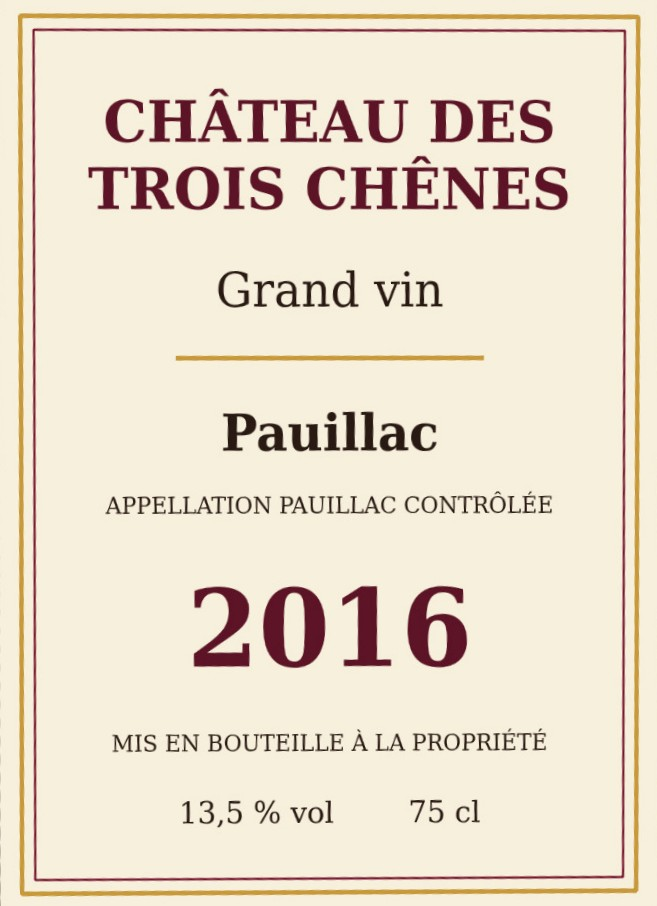
\includegraphics[width=\linewidth,height=42mm,keepaspectratio]{photo1.jpg}\end{minipage}\hfill\begin{minipage}[t]{0.75\linewidth}\vspace{0pt}
{\color{summit}Pauillac · Bordeaux · France · Red}\par
Bottles : 2 — Stated value : \textbf{\euro{}178.40}
\end{minipage}\par\smallskip
{\footnotesize\begin{xltabular}{\linewidth}{@{}>{\raggedright\arraybackslash}p{0.22\linewidth}>{\raggedright\arraybackslash}X>{\raggedright\arraybackslash}p{0.17\linewidth}>{\raggedleft\arraybackslash}p{0.19\linewidth}@{}}
\toprule \textbf{Location, format, code} & \textbf{Fill level, condition, case, provenance} & \textbf{Purchase} & \textbf{Value (date, source)} \\ \midrule \endhead
Cave de la maison de montagne › Étagère › Rayonnage (row 4, column 5)\newline Bottle\newline{\color{summit}\texttt{V85FCFBA971}} & IN --- Into neck (Excellent for its age)\newline Label : Perfect\newline Capsule : Intact\newline Carton & \euro{}89.20 · May 20, 2020 · Salon des vins & \textbf{\euro{}89.20}\newline {\color{summit}purchase price, May 20, 2020} \\ \midrule[0.2pt]
Cave de la maison › Mur nord › Casier A (row 5, column 7)\newline Bottle\newline{\color{summit}\texttt{V08B3BA0F10}} & IN --- Into neck (Excellent for its age)\newline Label : Perfect\newline Capsule : Intact\newline Carton & \euro{}89.20 · May 20, 2020 · Salon des vins & \textbf{\euro{}89.20}\newline {\color{summit}purchase price, May 20, 2020} \\ \midrule[0.2pt]
\bottomrule\end{xltabular}}
\section{Statement}
I certify that this inventory describes the bottles in my cellar at the date of this report.
\vspace{18mm}
\begin{tabularx}{\linewidth}{XX}
Place and date: \dots{}\dots{}\dots{}\dots{}\dots{}\dots{}\dots{} & Signature: \\ \end{tabularx}
\end{document}
